% 1964 全国卷第 3 题：x^4+1=0 的四根（矢量重绘）
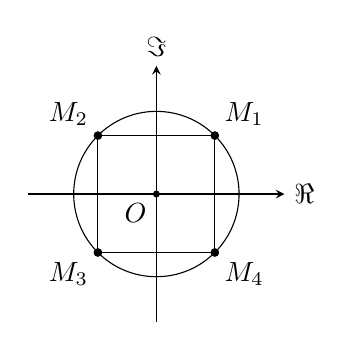
\begin{tikzpicture}[>=stealth,scale=1.05]
  \draw[->] (-1.55,0) -- (1.55,0) node[right] {$\Re$};
  \draw[->] (0,-1.55) -- (0,1.55) node[above] {$\Im$};
  \draw (0,0) circle (1);
  \coordinate (M1) at (0.707,0.707);
  \coordinate (M2) at (-0.707,0.707);
  \coordinate (M3) at (-0.707,-0.707);
  \coordinate (M4) at (0.707,-0.707);
  \draw (M1)--(M2)--(M3)--(M4)--cycle;
  \fill (M1) circle (1.5pt) node[above right] {$M_1$};
  \fill (M2) circle (1.5pt) node[above left] {$M_2$};
  \fill (M3) circle (1.5pt) node[below left] {$M_3$};
  \fill (M4) circle (1.5pt) node[below right] {$M_4$};
  \fill (0,0) circle (1.2pt) node[below left] {$O$};
\end{tikzpicture}
